% Overlay para o repositório andreghisleni/calculo-3-helice-circular.
% Use este main.tex na raiz do repositório e coloque as figuras em images/.
% O tema e os seus assets continuam em udesc/Latex-Beamer-UDESC-master/.
\documentclass{beamer}

\usepackage[utf8]{inputenc}
\usepackage[T1]{fontenc}
\usepackage[english,brazil]{babel}
\usepackage{amsmath,amssymb,booktabs,tabularx}
\usepackage{graphicx}
\usepackage{hyperref}
\usepackage{url}

% Localiza os arquivos do tema UDESC tanto ao compilar na raiz do repo
% quanto na pasta udesc/Latex-Beamer-UDESC-master/.
\graphicspath{{images/}{../../images/}{udesc/Latex-Beamer-UDESC-master/}}
\makeatletter
\def\input@path{{udesc/Latex-Beamer-UDESC-master/}{./}}
\makeatother
\usepackage{udesc}

\title[Busca por Cosseno]{Busca de Documentos com Similaridade por Cosseno}
\subtitle{Aplicação 1 — Obtenção de Informações: Revista}
\author[André Ghisleni Raimann]{André Ghisleni Raimann}
\institute[Álgebra Linear]{Álgebra Linear}
\date{2026}

\begin{document}

\begin{frame}
  \titlepage
\end{frame}

\section{Modelagem}

\begin{frame}{Da coleção de documentos à matriz}
  \begin{columns}[T]
    \begin{column}{0.55\textwidth}
      \begin{block}{Representação}
        \centering
        $A\in\mathbb{R}^{10\times 8}$
      \end{block}
      \begin{itemize}
        \item As dez linhas representam palavras-chave.
        \item As oito colunas representam módulos (documentos).
        \item A entrada $a_{ij}$ conta as ocorrências da palavra $i$ no módulo $j$.
      \end{itemize}
      \vspace{0.1cm}
      \small Recorte da matriz original — módulos M1 a M4:
      \begin{center}
        \scriptsize
        \begin{tabular}{lrrrr}
          \toprule
          Palavra & M1 & M2 & M3 & M4 \\
          \midrule
          determinantes & 0 & 6 & 3 & 0 \\
          ortogonalidade & 0 & 0 & 0 & 0 \\
          espaços & 0 & 0 & 5 & 2 \\
          vetor & 0 & 4 & 4 & 3 \\
          \bottomrule
        \end{tabular}
      \end{center}
    \end{column}
    \begin{column}{0.41\textwidth}
      \begin{alertblock}{A linguagem complica a busca}
        \textbf{Polissemia:} uma palavra pode ter sentidos diferentes.\par\medskip
        \textbf{Sinonímia:} o mesmo sentido pode aparecer em palavras distintas.
      \end{alertblock}
      O exemplo começa com contagem de frequências; essa etapa, sozinha, não resolve esses dois casos.
    \end{column}
  \end{columns}
\end{frame}

\section{Consulta}

\begin{frame}{A consulta também é um vetor}
  A busca usa três palavras-chave: \textbf{ortogonalidade}, \textbf{espaços} e \textbf{vetor}.
  \vspace{0.35cm}
  \begin{block}{Vetor unitário de busca}
    \[
      \boldsymbol{x}=\frac{1}{\sqrt{3}}
      (0,0,0,0,0,1,1,0,0,1)^{\mathsf T},
      \qquad \|\boldsymbol{x}\|=1.
    \]
  \end{block}
  \begin{itemize}
    \item As posições diferentes de zero correspondem exatamente aos três termos da consulta.
    \item O fator $1/\sqrt{3}$ dá o mesmo peso a cada termo e deixa o vetor com comprimento 1.
  \end{itemize}
\end{frame}

\section{Similaridade}

\begin{frame}{Normalizar e comparar direções}
  \begin{columns}[T]
    \begin{column}{0.46\textwidth}
      Cada coluna de frequências $\boldsymbol{a}_j$ é transformada em um vetor unitário:
      \[
        \boldsymbol{q}_j=\frac{\boldsymbol{a}_j}{\|\boldsymbol{a}_j\|}.
      \]
      O escore do módulo $j$ é
      \[
        y_j=\boldsymbol{q}_j^{\mathsf T}\boldsymbol{x}=\cos\theta_j.
      \]
      \begin{itemize}
        \item Direções próximas produzem cosseno maior.
        \item Vetores ortogonais produzem escore zero.
      \end{itemize}
    \end{column}
    \begin{column}{0.52\textwidth}
      \centering
      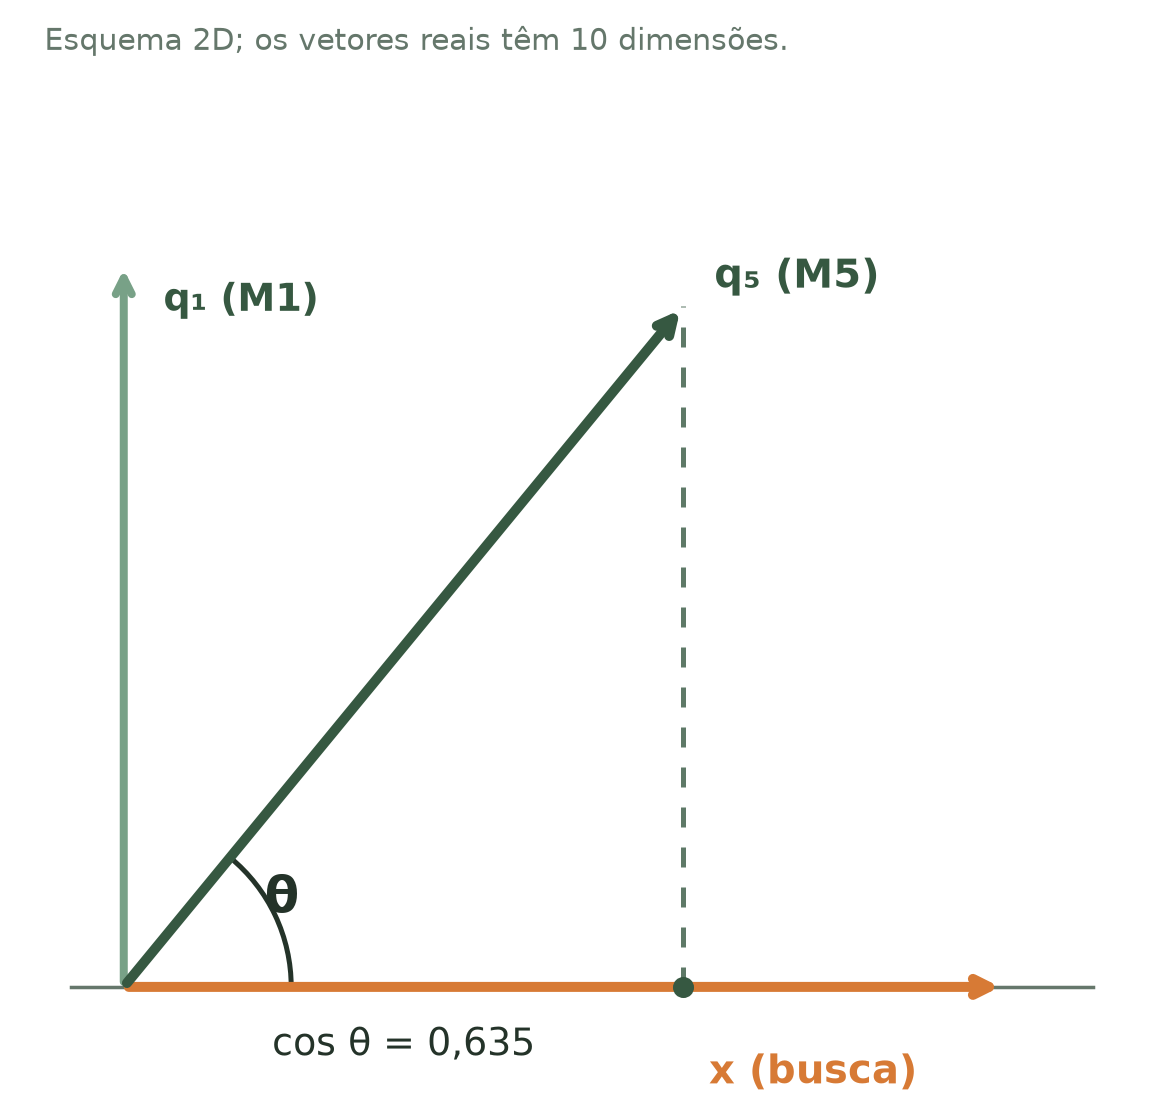
\includegraphics[width=0.97\linewidth,height=0.60\textheight,keepaspectratio]{geometria_cosseno.png}
    \end{column}
  \end{columns}
\end{frame}

\begin{frame}{O processo da busca}
  \begin{center}
    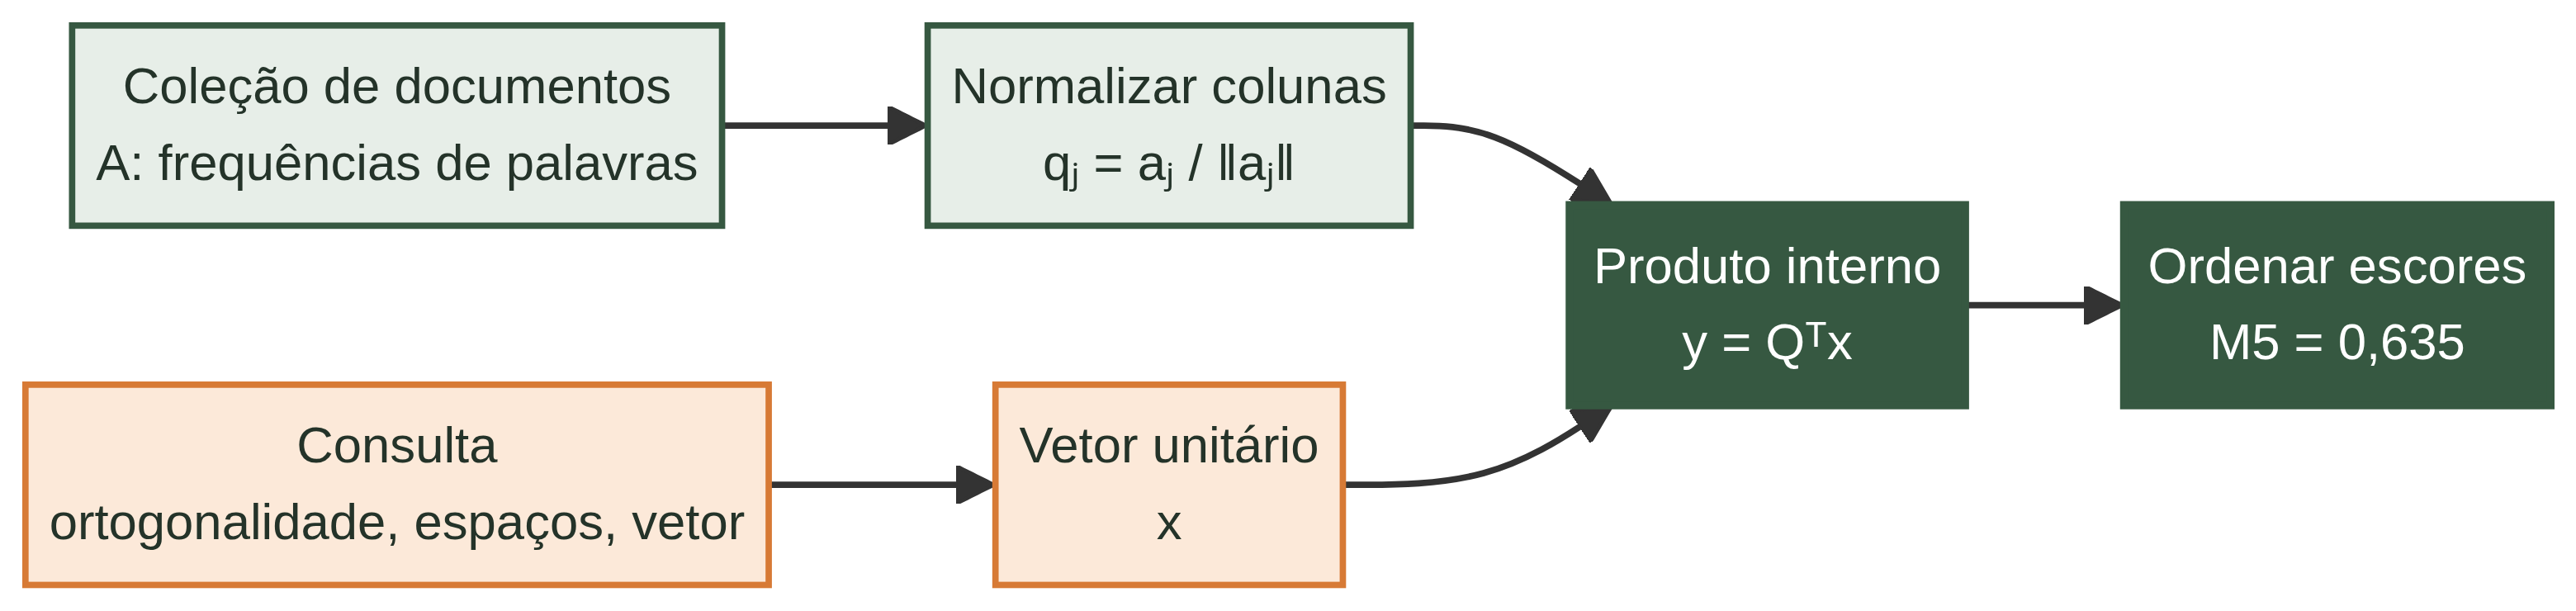
\includegraphics[width=0.97\textwidth,height=0.43\textheight,keepaspectratio]{fluxo_busca.png}
  \end{center}
  \vspace{0.15cm}
  \begin{block}{Em uma linha}
    \centering
    Frequências $\longrightarrow$ normalização $\longrightarrow$ produto interno $\longrightarrow$ ranking.
  \end{block}
\end{frame}

\section{Resultados}

\begin{frame}{Os módulos mais próximos da consulta}
  \begin{center}
    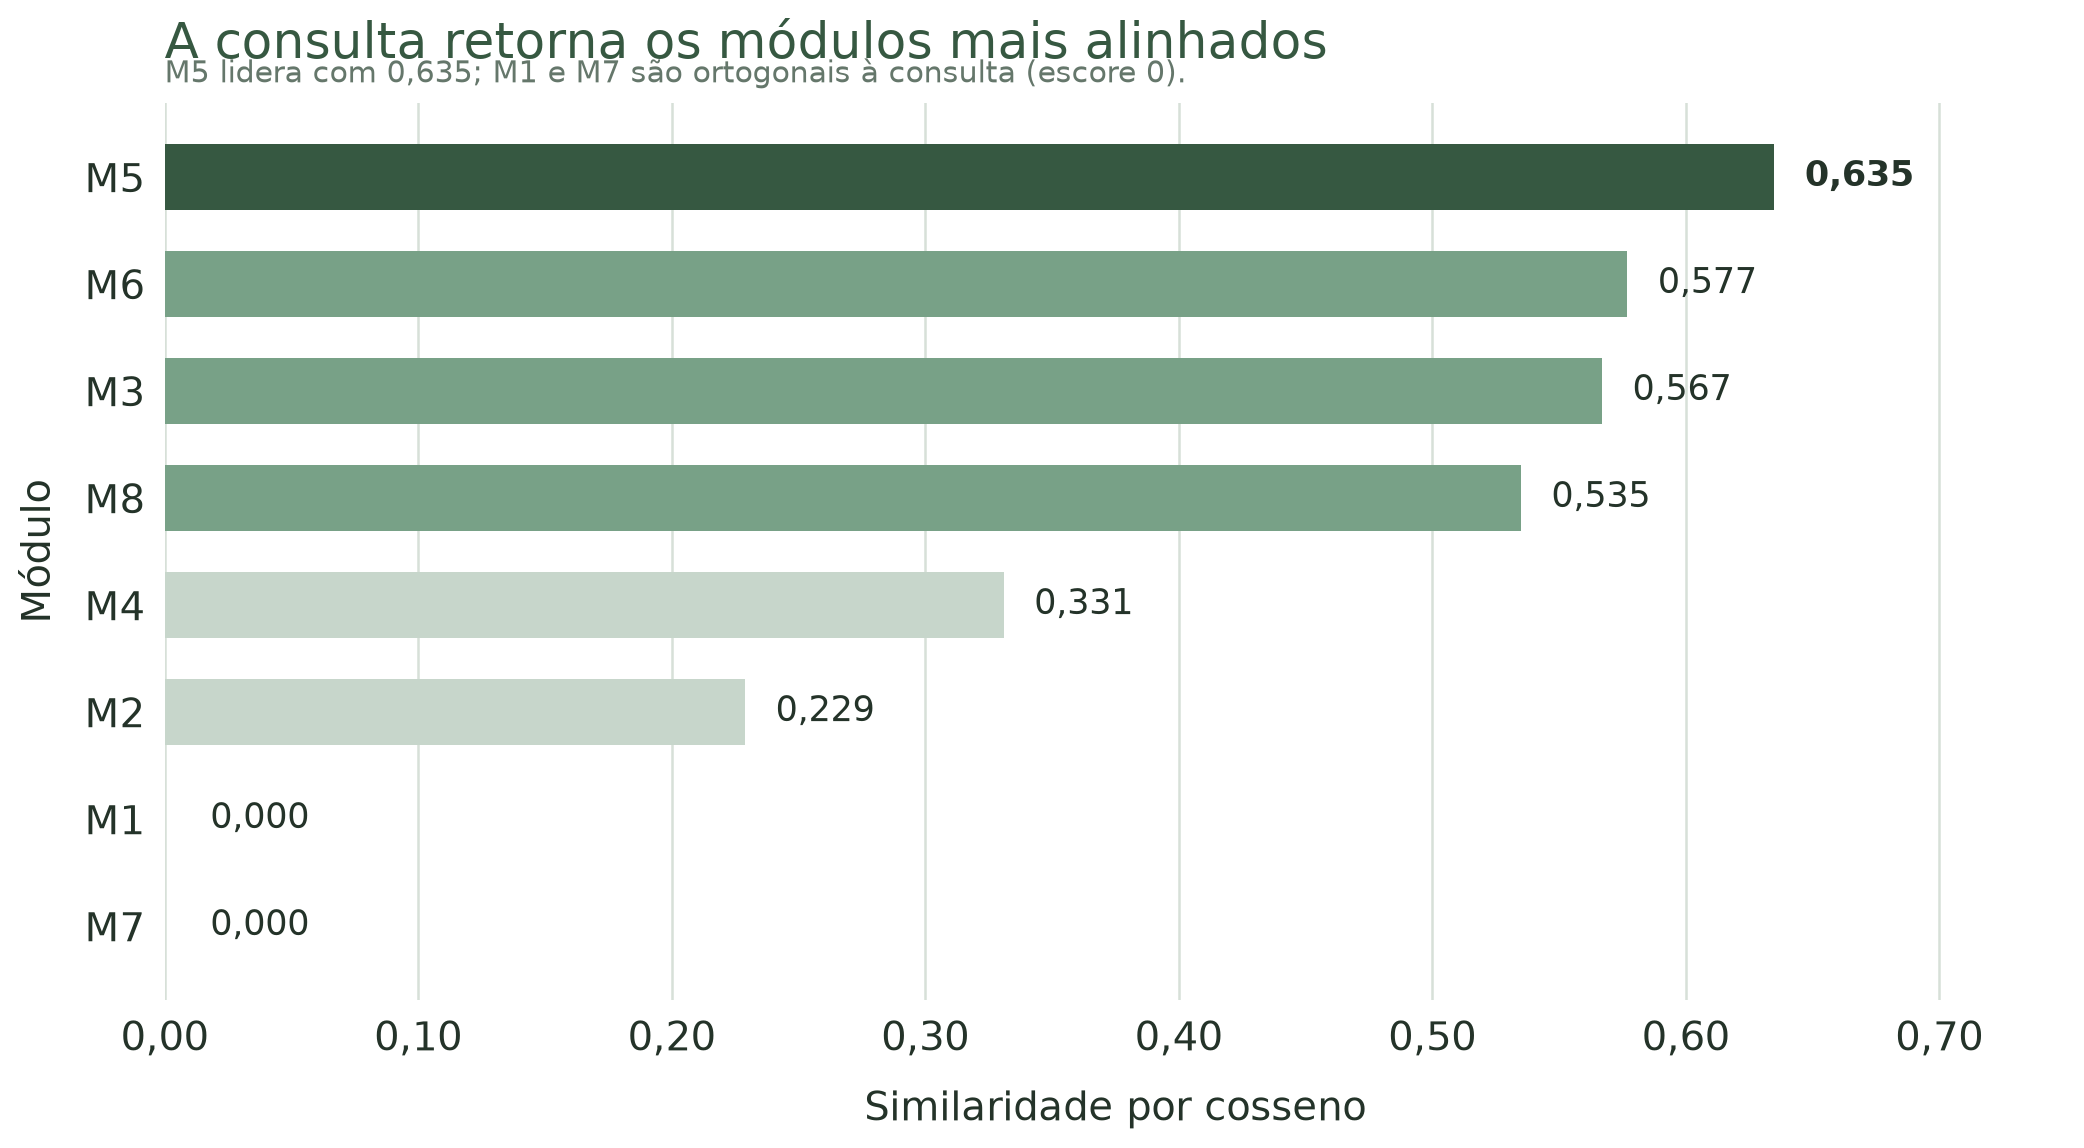
\includegraphics[width=0.94\textwidth,height=0.66\textheight,keepaspectratio]{ranking_modulos.png}
  \end{center}
  \begin{center}
    \small A consulta é mais alinhada com M5; M6, M3 e M8 vêm logo depois.
  \end{center}
\end{frame}

\begin{frame}{Por que o módulo M5 lidera?}
  No vetor normalizado de M5, as componentes de \textit{ortogonalidade}, \textit{espaços} e \textit{vetor} são $0{,}400$, $0{,}300$ e $0{,}400$.
  \vspace{0.35cm}
  \begin{block}{Produto interno com a consulta}
    \[
      \boldsymbol{q}_5^{\mathsf T}\boldsymbol{x}
      =\frac{0{,}400+0{,}300+0{,}400}{\sqrt{3}}
      \approx 0{,}635.
    \]
  \end{block}
  \begin{alertblock}{Interpretação}
    $0{,}635$ é o maior escore entre os oito módulos. É uma medida geométrica para ordenar documentos, não uma porcentagem de relevância.
  \end{alertblock}
\end{frame}

\section{Conclusão}

\begin{frame}{O alcance e os limites do exemplo}
  \begin{itemize}
    \item A matriz de frequências permite ordenar os documentos pela direção dos vetores.
    \item M1 e M7 não contêm nenhum dos três termos buscados; por isso, seus vetores são ortogonais à consulta e recebem escore 0.
    \item A contagem literal não reconhece sinônimos nem distingue automaticamente sentidos diferentes de uma palavra.
  \end{itemize}
  \begin{block}{Próximo passo citado por Leon}
    A indexação semântica latente (ISL), baseada em decomposição por valores singulares, pode ajudar a lidar com polissemia e sinonímia.
  \end{block}
  \vfill
  {\tiny Fonte: Steven J. Leon, \textit{Álgebra Linear com Aplicações}, cap. 5, Aplicação 1, pp. 191--193 (PDF, pp. 197--199).}
\end{frame}

\end{document}
